\documentclass[11pt]{article}
\usepackage{geometry}                
\geometry{letterpaper} 


\usepackage{graphicx}
\usepackage{amssymb}
\usepackage{epstopdf}
\usepackage{natbib}
\usepackage{amssymb, amsmath}
\usepackage{hyperref}
\DeclareGraphicsRule{.tif}{png}{.png}{`convert #1 `dirname #1`/`basename #1 .tif`.png}
\usepackage{pdfpages}

%\title{The Swiss Train Network}
%\author{Mario Vontobel, Elias Rieder}
%\date{date} 

\begin{document}


\thispagestyle{empty}

\begin{center}
\includegraphics[width=5cm]{ETHlogo.eps}

\bigskip


\bigskip


\bigskip


\LARGE{ 	Lecture with Computer Exercises:\\ }
\LARGE{ Modelling and Simulating Social Systems with MATLAB\\}

\bigskip

\bigskip

\small{Project Report}\\

\bigskip

\bigskip

\bigskip

\bigskip


\begin{tabular}{|c|}
\hline
\\
\textbf{\LARGE{The Swiss Train Network}}\\
\\
\hline
\end{tabular}
\bigskip

\bigskip

\bigskip

\LARGE{Mario Vontobel \& Elias Rieder}



\bigskip

\bigskip

\bigskip

\bigskip

\bigskip

\bigskip

\bigskip

\bigskip

Zurich\\
Dec 2014\\

\end{center}



\newpage

%%%%%%%%%%%%%%%%%%%%%%%%%%%%%%%%%%%%%%%%%%%%%%%%%

\newpage

\includegraphics[scale=0.7]{agreement_download}

\newpage

%%%%%%%%%%%%%%%%%%%%%%%%%%%%%%%%%%%%%%%



% IMPORTANT
% you MUST include the ETH declaration of originality here; it is available for download on the course website or at http://www.ethz.ch/faculty/exams/plagiarism/index_EN; it can be printed as pdf and should be filled out in handwriting

\newpage

\includegraphics[scale=0.7]{plagiat_ETH}

\newpage


%%%%%%%%%% Table of content %%%%%%%%%%%%%%%%%

\tableofcontents

\newpage

%%%%%%%%%%%%%%%%%%%%%%%%%%%%%%%%%%%%%%%



\section{Abstract}

This project looks at the Swiss train network. It investigates the flow of people in this transport system, which is quite important for this country. The goal was to find relations between properties like capacity, amount of people travelling, delay and fragility. On one hand this is approached by a general theoretical model. On the other hand by real data. These two methods lead to a model of the Swiss train  network. On the basis of this model the properties are analyzed. The two approaches merge at the end and allow us to make some statements about the quality of the theoretical model.
 

\section{Individual contributions}

We made the whole work in a close teamwork. It was made in continuous exchange and by inspiring each other. Mario set the focus a bit more on coding. Elias on the Concepts and Data. You can see all the steps, code and data on github. Mario has the username mlv19 and Elias is EleSwag.\newline

\url{https://github.com/EleSwag/Elias-und-Mario}

\section{Introduction and Motivations}

\subsection{Idea and Motivation}


Every day we travel from our homes to Z\"urich. The train in the morning is often very crowded and a lot of delays occur. This circumstance made us think about how the train network works and how you could handle such capacity shortages better. 
So the general idea was to model the Swiss train network and then look at its properties. This may sound like a very general question. As you can imagine, the whole schedule is quiet complex and consists of a lot of data. At this point we didn't know how much and what kind of data we would have access to. That is why the we kept the general. We heard in our lecture that the number of inhabitants has an influence on the amount of traffic. The type of model using this approach is called Gravity model.

So we had two approaches to start with: The Gravity model, witch will be explained in detail after, and the effort getting real data.

Because our interest in the problem came from observations in our everyday life, it was very important to us, that our work would have a strong connection to reality. To make this happen, we wrote a mail to SBB, the Swiss rail company, and asked them for real Data. Since we did not know if we would get the data we had two make two plans.

The first possibility would have been getting a rich data set from SBB. Complex models considering the frequency, speed and capacity of the trains and the resulting connections would be possible. In this case the question of capacity and load, and resilience were very interesting questions.

The second, alternative possibility was getting nothing. But with the gravity model we could be sure to have an angle even  without data. This was kind of a backup plan. Of course the questions would have to be asked way more general  

So the question that draws through both approaches is:\newline 
\textbf{How do you make a model that allows us to approximate the flow of people in the Swiss train network and and enables us to make statements about the traffic flow, the capacity and the resilience of it?}    


\section{Description of the Model}
\subsection{The classical gravity model}
In  social science -especially in international economics in trade simulations- it is a common and well established approach to simulate flows with a gravity model. The motivation behind it is the physical gravity force. This is defined by $F_G:=G\frac{m_1 m_2}{r^2}$, where G is the gravity constant, $m_i$ is the mass of the  i-Th body for $i=1,2$ and r is the distance between body 1 and body 2.


This leads to the general ansatz$_2$:
\begin{align*}
F_{ij}=G\frac{M_i^{\beta_1}M_j^{\beta_2}}{D_{ij}^{\beta_3}}
\end{align*}

We transferred this idea to our situation by identifying the mass of a city to its population$_3$ and used different definitions of distance. We dropped the constant at the beginning since we normalized the resulting flow anyway. As exponents we have chosen $\beta_1=\beta_2=\beta_3=1$ since with no experience this was as suitable as anything else.\newline

\subsection{The development of the gravity model}
In our first approach we took the 10  biggest cities in regard of the number of inhabitants plus two additional ones (Olten and Arthgoldau) which are well-known important nodes$_4$ of the real network.

We wondered if they would also become as important  in our gravity model as in the real network.\newline

To make the network more realistic we have looked up all real connections between the cities on the online train schedule$_5$. Our criterion was that two nodes are connected if there exists a direct train connection between them. With this idea we didn't end with a fully-connected network which is from our point of view more realistic to simulate the direct flow between cities.

\begin{figure}
\centering
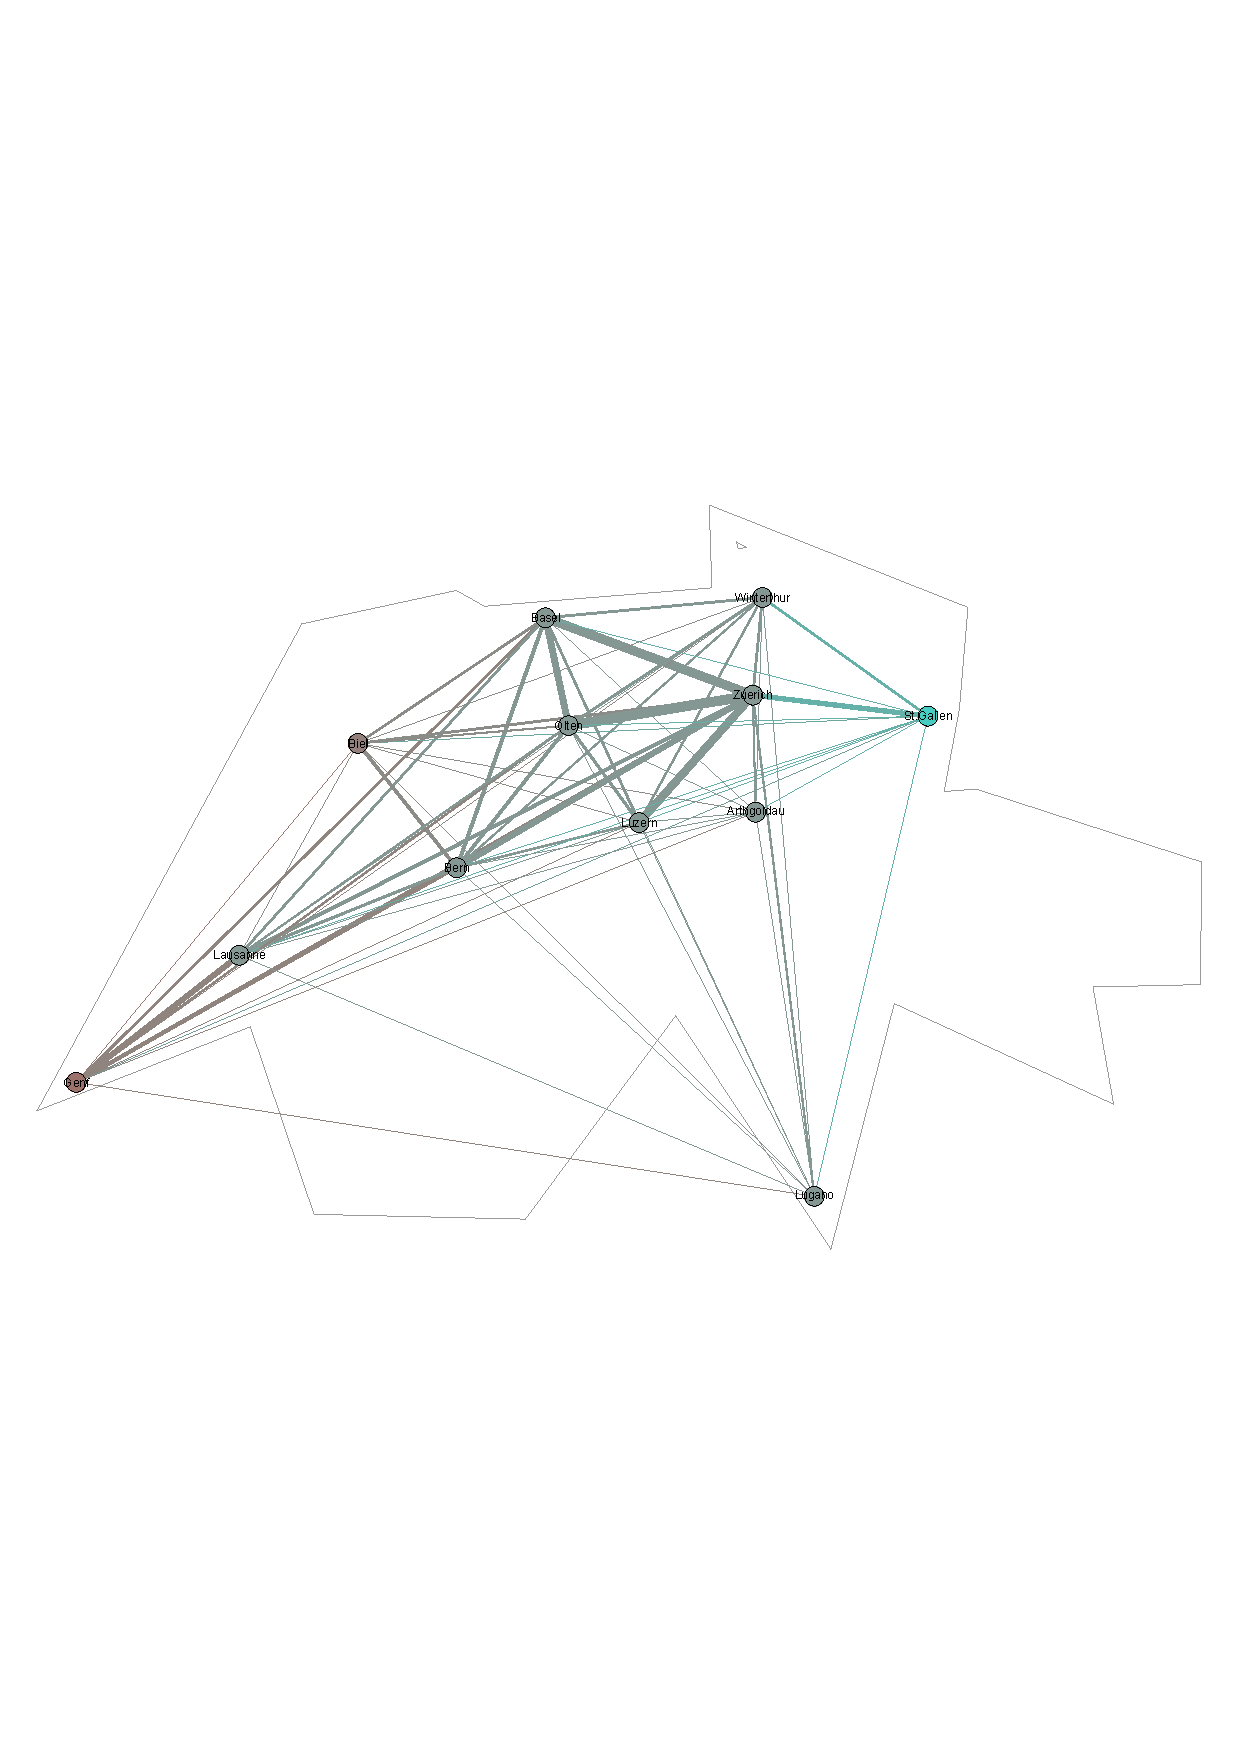
\includegraphics[scale=0.25]{switzerland_network1}
\hfill
\includegraphics[scale=0.08]{Map}
 \caption{Left:Gravity model 1 (full connected): Model of the 10 biggest cities plus two additional one. Layout by gephi with respecting geographical position. Right: Corresponding map with connections between the 12 biggest cities}
\end{figure}

This was the first network we plotted. While looking at the picture it was striking that the network didn't at all cover the hole country. Especially the south-west part was unattended. So we extended the number of cities to 20 and kept the two additional ones from the beginning.


\subsection{Comment on the distance in the gravity model}
In the general gravity model we used geographical distance as the distance indicator. But we thought it would also be reasonable to use the time it takes to travel from one city to the other as the distance indicator. The idea was that this also takes in account if there is obstacle like a mountain or a lake between the cities. The danger here is, that the network is approximated with the existing network. Anyway we omitted that later because with the number of connection the investment grow nearly immeasurable. Also the time connection was not well-defined any more. In the sense that there were different times for the same connection.

\subsection{The Data approach}

As mentioned at the beginning the second way looking at our network was real data. Unfortunately the search for data turned out to be quiet difficult. We contacted SBB for data, but in a big company like this things are taking very long. When we finally got in contact with the right persons$_{8-10}$, there was just to less time left to process all and we could not get all the data we would have liked. Especially data about the load of the network and the capacity seems to be very sensitive. But the people from SBB were very kind and gave us what they could. They sent us a public link$_{11}$ were you can download the whole timetable in Gtfs-Format (General Transit Feed Specification). Sadly we could not involve that, because of the already mentioned time shortness. We also could sent several questions to one of their network specialists$_{10}$. Especially the numbers of people boarding and de-boarding for a few big cities made us curious. This was a number we may could relate with our gravity models.  


\section{Implementation}
\textbf{In general we tried to be as specific as possible with the annotation of the functions in matlab}

We created a script called data1 which contains all our relevant data. As already mentioned, all data and code is on GitHub$_1$.

\subsection{Network flow-function}
First we implemented a general network function which applies the theory mentioned in the description of the model to an adjacency matrix of a network. This function gave another adjacency matrix back with the simulated flow. This function would also run for every other gravity model based simulation.\newline

For the distance based gravity function we also needed the geographical distance. For that purpose we added to each city its coordinates$_{15}$ and computed the distance between each city by just applying Pythagoras. Since Switzerland is a small country we did not take in account that the earth is a sphere and just approximated as if it was a plane. The function gives again an adjacency matrix back, where the ij-th entry is the distance between the point at coordinates i and the point at coordinates j.


\subsection{Visualization}
In the lectures it was recommended to use gephi. So some of our pictures are made with it. But a huge disadvantage of gephi is that it is rather complicated to respect geographical position if one uses an adjacency  matrix to represent the network. In figure 1 we placed the cities by hand.

But since this is rather complicated we also wrote function in matlab to illustrate a network given in a adjacency matrix. The result isn't as pretty as in gephi but the geographical representation was more straight forward.


\begin{figure}
\centering
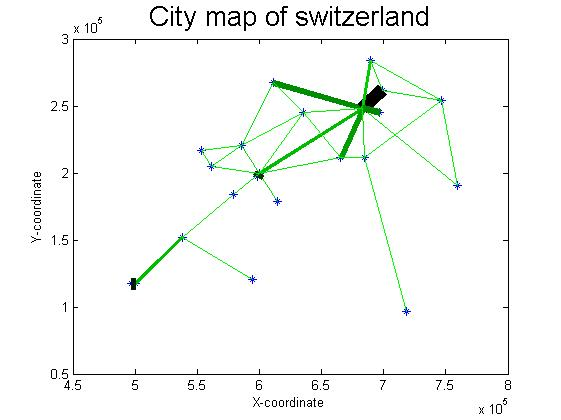
\includegraphics[scale=0.5]{switzerland_network2}
 \caption{Gravity model 2: Model of the 20 biggest cities plus two additional one. Layout by matlab. The strength of a connection is emphasized by the thickness as well as the depth of the color from the line. The coordinates are given in the Swiss coordinate system/Swiss grid$_{15}$}
\end{figure}

\subsection{Investigation-function}
To investigate the network we strongly relayed on the paper 'Complexity in human transportation networks: a comparative analysis of worldwide air transportation and global cargo-ship movements'.
We implemented the shortest distance function described on page 592/593. At the beginning we had a hard time to find the right function but then Mario remembered that he had in the fall semester 2013 a lecture$_{7}$ on algorithm and complexity. Mostly the lecture was about theory from trees (special case of a graph) but there was also a part on general graph theory. In that part was the 'Floyd-Warshall'-algorithm which does exactly what we needed. Which means shortest paths between all nodes.
The notes also allowed as to implement a function which checks if a network is still connected by using a 'depth-first-search'-algorithm.




\section{Simulation Results and Discussion}
\textbf{Note}: When the x-axis is labeled cities with number this is always referring to our city-vector, which is sorted by the size of its population (Zuerich, Genf, Basel, Lausanne, Bern, Winterthur, Luzern, St.Gallen, Lugano, Biel, Thun, Koeniz, Chaux-de-Fonds, Schaffhausen, Freiburg, Chur, Neuenburg, Vernier, Uster, Sion, Olten, Arthgoldau)$_{3}$


\subsection{General Network Parameters}
\begin{figure}[h]
\begin{tabular}{c|c|c|c|c|c|c|c|c|c|}
 & N & L & $\sigma$ & $\phi$ & $d_T$ & $\langle r\rangle$ & 
 $\langle w\rangle$ & $\langle F\rangle$&$\langle k\rangle$ \\\hline
 Full-connected & 22 & 231 &0.9545&1& 0.8413& $2.6604e+07$&0.0275&0.5781& 21\\\hline
 
 Connected & 22 & 34 &    0.1405&2.9134& 11.0154&$2.6028e+07$&0.1037&0.3215& 3.1364\\\hline
\end{tabular}
\caption{N is the Number of Nodes, L is the number of connections, the network connectivity $\sigma=2\frac{L}{N^2}$, $\phi$ is the betweenness centrality, $d_T$ is the average shortest path length,  $\langle r\rangle$ is the average geographical distance  
 $\langle w\rangle$, is the average node weight $\langle F\rangle$, is the average flow per city and $\langle k\rangle$ is the average node degree}
\end{figure}

The full connected network is the general network from the gravity function, where everything is connected. The connected network is the one developed by us (only connected if there is a direct link).

Beside other obvious observations, it is quiet intuitive, that $\phi$ rises with less links between nodes. One surprisingly observation was that although that the mean link rises with a factor 5, the average node flow only sinks by a factor 2.\newline

To investigate more network parameters like node distribution more nodes would be needed. Since in our model each node weight or node degree appears nearly only once.

The detailed definitions of these parameters are described in reference 6 


\subsection{Network flow}

To determine how powerful the gravity model is, you have to be very careful about your question. It strongly depends on your point of view. If you want to get an impression of the amount of traffic of the 10 biggest cities in Switzerland, you might get quiet good results. But if you slightly change your point of view and ask yourself in which cities of Switzerland a big amount of traffic occurs, your gravity model might not be overall correct. 

We tried to get an idea how our model response to reality. For that we brought our (de-)boarding into play. Because the flows in our model are undirected, the sum of all flows in a node should be equal to the people boarding plus the people deboarding. To check if how good our calculated flow match with the real flow, we divided one by the other to get a proportion. We did this for both of our models. You can see in the graphics that the cities with high population are approximated with a similar relative factor. But  for important nodes of the real network both gravity models fail. Have a look at Olten (small number of inhabitants big amount of traffic). Even one of the seat critical trains$_{12}$, departs from Olten (train were you might have to stand). But precisely for further investigations on capacity, these flows would be important.


\begin{figure}[h]
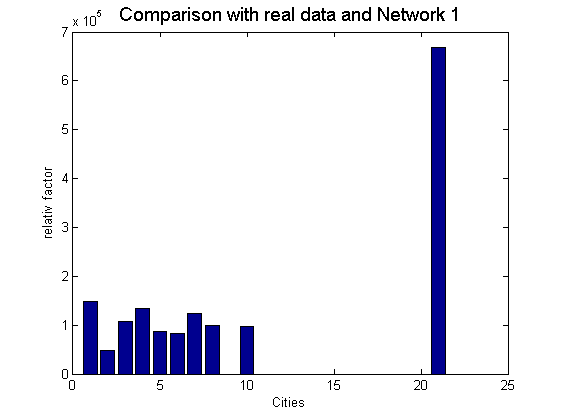
\includegraphics[scale=0.4]{compare1}
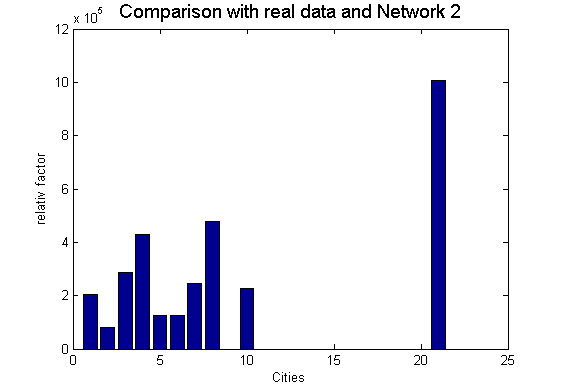
\includegraphics[scale=0.4]{compare2}
 \caption{Network is the full connected gravity model based model and network 2 is the one with the connections from the schedule. The relative factor $=\frac{\text{Real data}}{\text{network flow per City}}$.The network flow per city is calculated for each city by summing over the columns.}
\end{figure}



The other, pretty obvious weakness of the gravity model are time variable flows. We learned, that this is a quiet important aspect if you want to find out something about capacity of this network. The fastest growing traffic flows in the network are the peaks in the rush-hour$_{14}$.






\subsection{Resilience}

The resilience of a network can be investigated by looking at a few parameters. One of them is the change of the longest relative distance when a node is removed. We applied this to two of our network matrices. One was the full connected and the other the connected gravity model. We were interested if the two models would behave similar or not. Network one was besides Z\"urich very resilience resistant meanwhile network 2 also had nodes where the network was not connected anymore if removed and in general also more sensitive. A remarkable observation was that in the network 2 the diameter $\phi$ falls extremely when Lugano is removed.


 
Besides that SBB assured$_{13}$ us they have replacement train at important nodes.

\begin{figure}
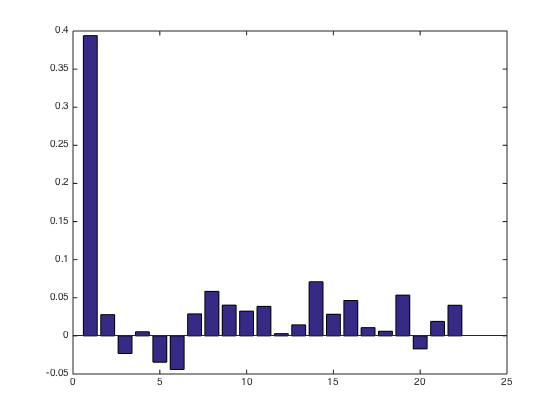
\includegraphics[scale=0.4]{fullConnedtedShortestNetworkDistanceChange}
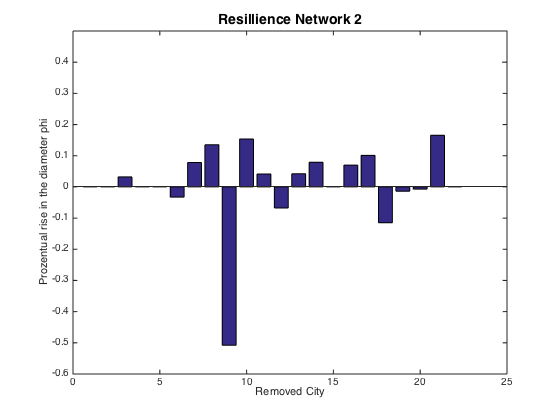
\includegraphics[scale=0.4]{connectedNetworkDistanceChange}
 \caption{Change of the shortest distance if a node is removed for the full connected gravity model (Network 1) and the connected one (Network 2). For network 2 zero means that the network was not connected anymore}
\end{figure}


\subsection{Capacity}

Unfortunately none of our approaches could answer our questions about capacity. The Gravity model can give Information about the amount of traffic, but it does not tells anything about how big this flows can get. What SBB told us is, how they deal with it: "If the route allows it, the train is maid as long as possible. All Platforms where the train stops have to be long enough. As additional action additional trains are added during the rush our...Alternatively the rolling stock can be optimized. On routes with little space, rolling stock with high capacity is used. If all these actions don't suffice, an extension is required"$_{13}$. One other thing they mentioned is, that their trying to foster flexible work time and home offices. Their doing this by negotiating with other big employers$_{9}$. This all seems all to be aimed at decreasing the rush hour peaks, not at handling them. Another thing they mentioned is, that with higher frequencies and shorter travel times higher the attractiveness of line. Which leads back to higher demands and more traffic, a vicious circle.




\section{Summary and Outlook}

The model of the Swiss train network had its strength and weaknesses. Our goal to model the Swiss train network was maybe aimed a bit high. We could not answer our questions about resilience and capacity as detailed as desired. 

The gravity model gives in general a good approximation for the flow of the cities besides important nodes in the real system like Olten, which have not a very huge population. Therefore the gravity model is good to approximate the flow of big cities. But this also means you will not find other high flows in the network. So the question for important nodes can not be modeled with a gravity approach.

One way to receive another flow would be to change the parameters $\beta_1,\beta_2,\beta_3$ in the gravity function. So one could take the geographical distance more in account than the size of population for example. \newline

Our investigations on resilience has shown that the real network is probably not as resistant as the general gravity model. But to real test the network on resilience one would need more nodes since our present network gets disconnected quite early. This would also allow to look at node distribution and other parameters. This could may be arrived with the Gtfs-files. Which would also lead to new networks which may have a more realistic flow.



The answers from SBB also let us suppose that they also try to solve problems in the network with reducing the demand of traffic. So they try to regulate the flow more with economic incentives than with improving or changing the network structure.

We found out quite interesting things about the Swiss train network and some interesting trails for further research.\newline

Another aspect who would be worth investigating are the rush hour peaks. Maybe it would be possible to approach them with differential equations, but it seems to become very complex there. Even the network specialist from SBB could not give us a general answer what the demands for a network are to handle peaks efficient.








\newpage


\section{References}
\begin{itemize}
\item[1.] Projectfolder: \url{http://Github.com/EleSwag/Elias-und-Mario} 

(all code and files are accessible here).\newline
\item[2.] Gravity Model \url{http://en.wikipedia.org/wiki/Gravity_model}\newline
\item[3.]List of Cities\url{http://de.wikipedia.org/wiki/Liste_der_Städte_in_der_Schweiz}\newline
\item[4.] Important Train Nodes \url{http://de.wikipedia.org/wiki/Eisenbahnknoten/\#Schweiz}\newline
\item[5.] SBB online timetable \url{http://www.sbb.ch/fahrplan.html}\newline

\item[6.] O. Woolley-Meza, C. Thiemann, D.Grady, J.J. Lee, H. Seebens, B. Blasius and D. Brockmann: Complexity in human transportation networks: a comparative analysis of worldwide air transportation and global cargo-ship movements?\newline
\item[7.] Vorlesung Algorithmen und Komplexität Angelika Steger ETH Z\"urich\newline



SBB Correspondence (all in github)\newline

\item[8.] Werner Nuber\newline
Director Senior Advisor\newline
Schweizerische Bundesbahnen SBB\newline
\item[9.] Matthias M\"uller\newline
Communication passenger traffic\newline
Schweizerische Bundesbahnen SBB\newline
\item[10.] Nadine Ruch\newline
Passenger traffic, corporate development,
demand development \newline
Schweizerische Bundesbahnen SBB\newline

SBB Data\newline

\item[11.] Link for timetable Data \url{http://gtfs.geops.ch}\newline
\item[12.] Seat critical trains (Appendix)\newline
\item[13.] Answers from Nadine Ruch from SBB (Appendix)\newline

\item[14.] SBB Konzernlagebericht 2013 page 7 section 5\url{http://geschaeftsbericht.sbb.ch/fileadmin/user_upload/Downloads/SBB_Konzernlagebericht_GBNB_2013.pdf}\newline

\item[15.]Swiss Grid \url{http://en.wikipedia.org/wiki/Swiss_coordinate_system}
\end{itemize}

\newpage

\section{Appendix}

\subsection{Seat critical trains}


\begin{figure}[h]
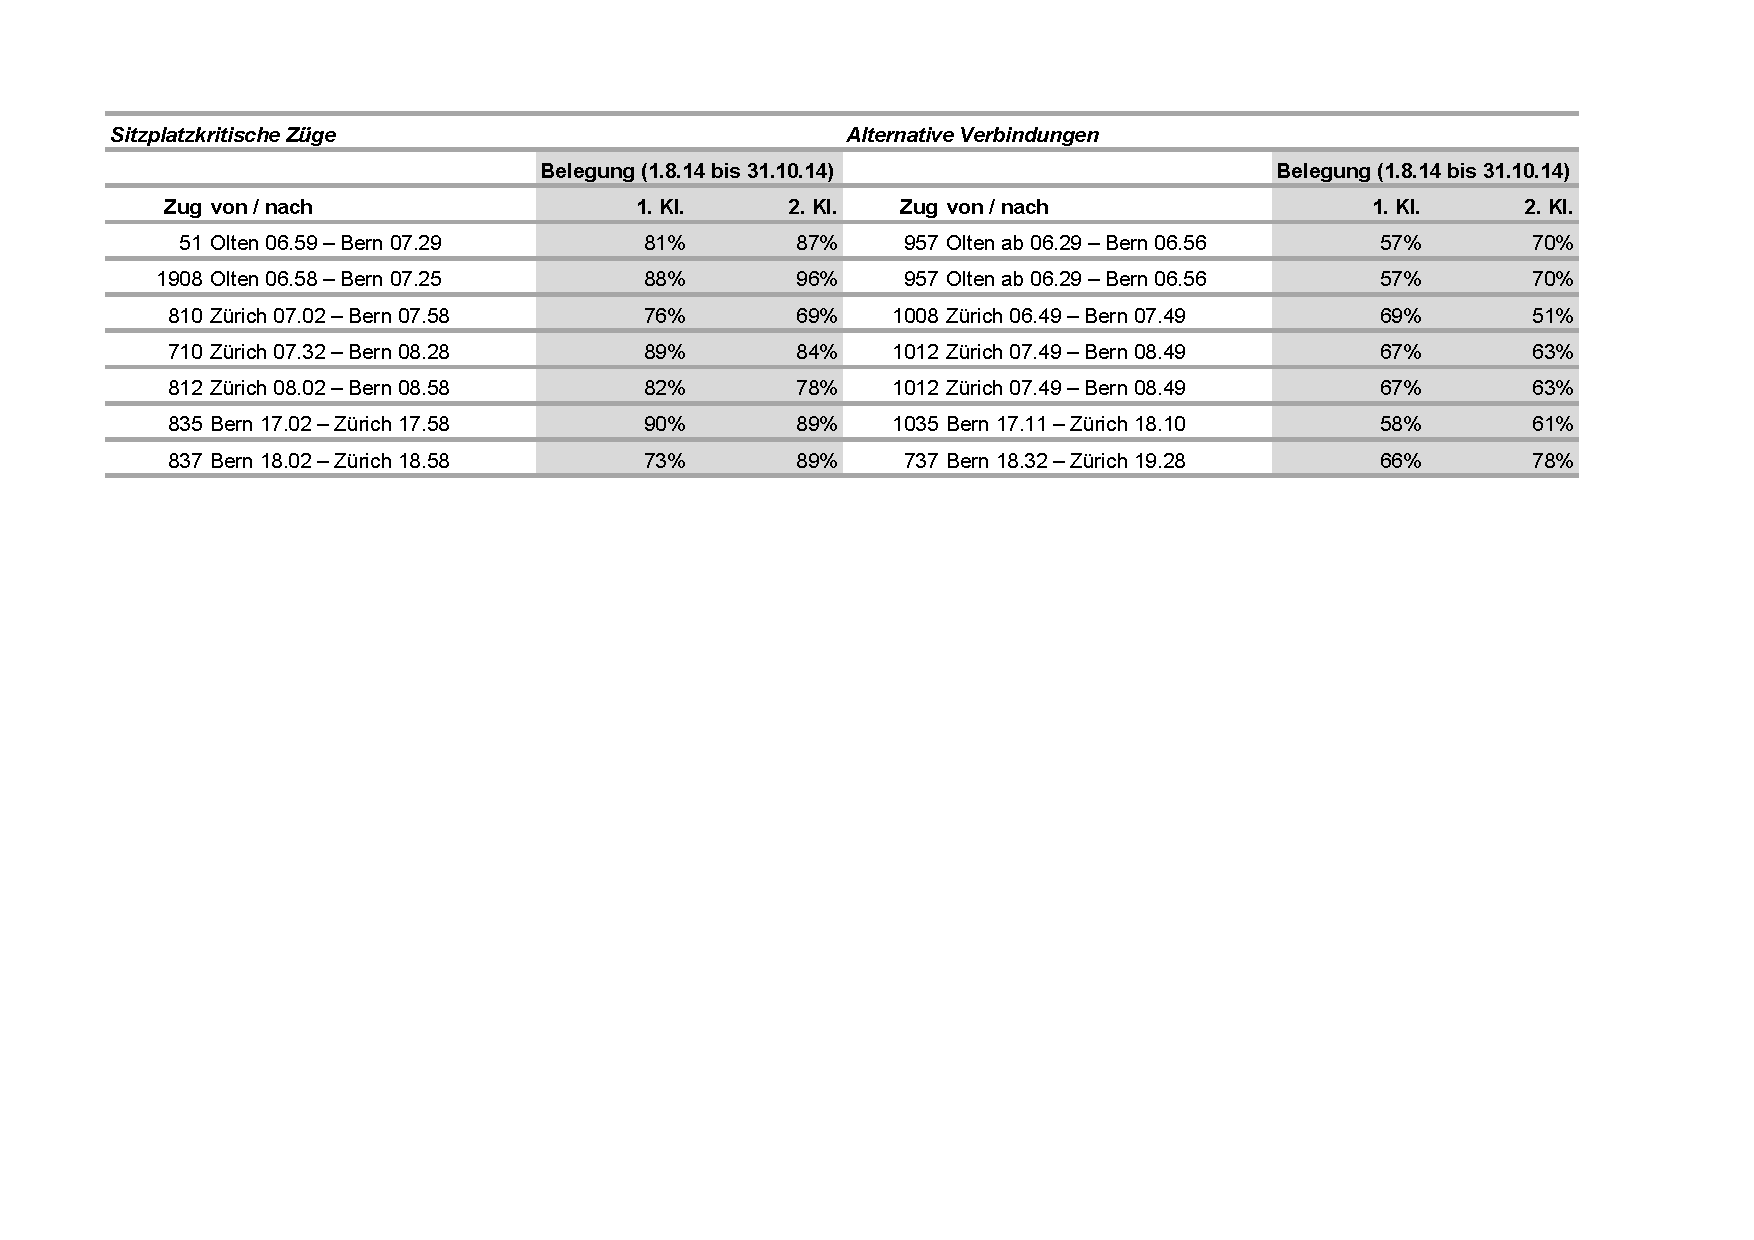
\includepdf[pages={1},scale=0.8]{HVZ_Reporting_Auslastung.pdf}
\end{figure}
\newpage
\subsection{Answers from Nadine Ruch from SBB}
\begin{figure}[h]

\includepdf[pages={1},scale=0.8]{Answers_SBB_(English_translated).pdf}
\end{figure}

\newpage

\subsection{mail boarding/deboarding}

\begin{figure}[h]
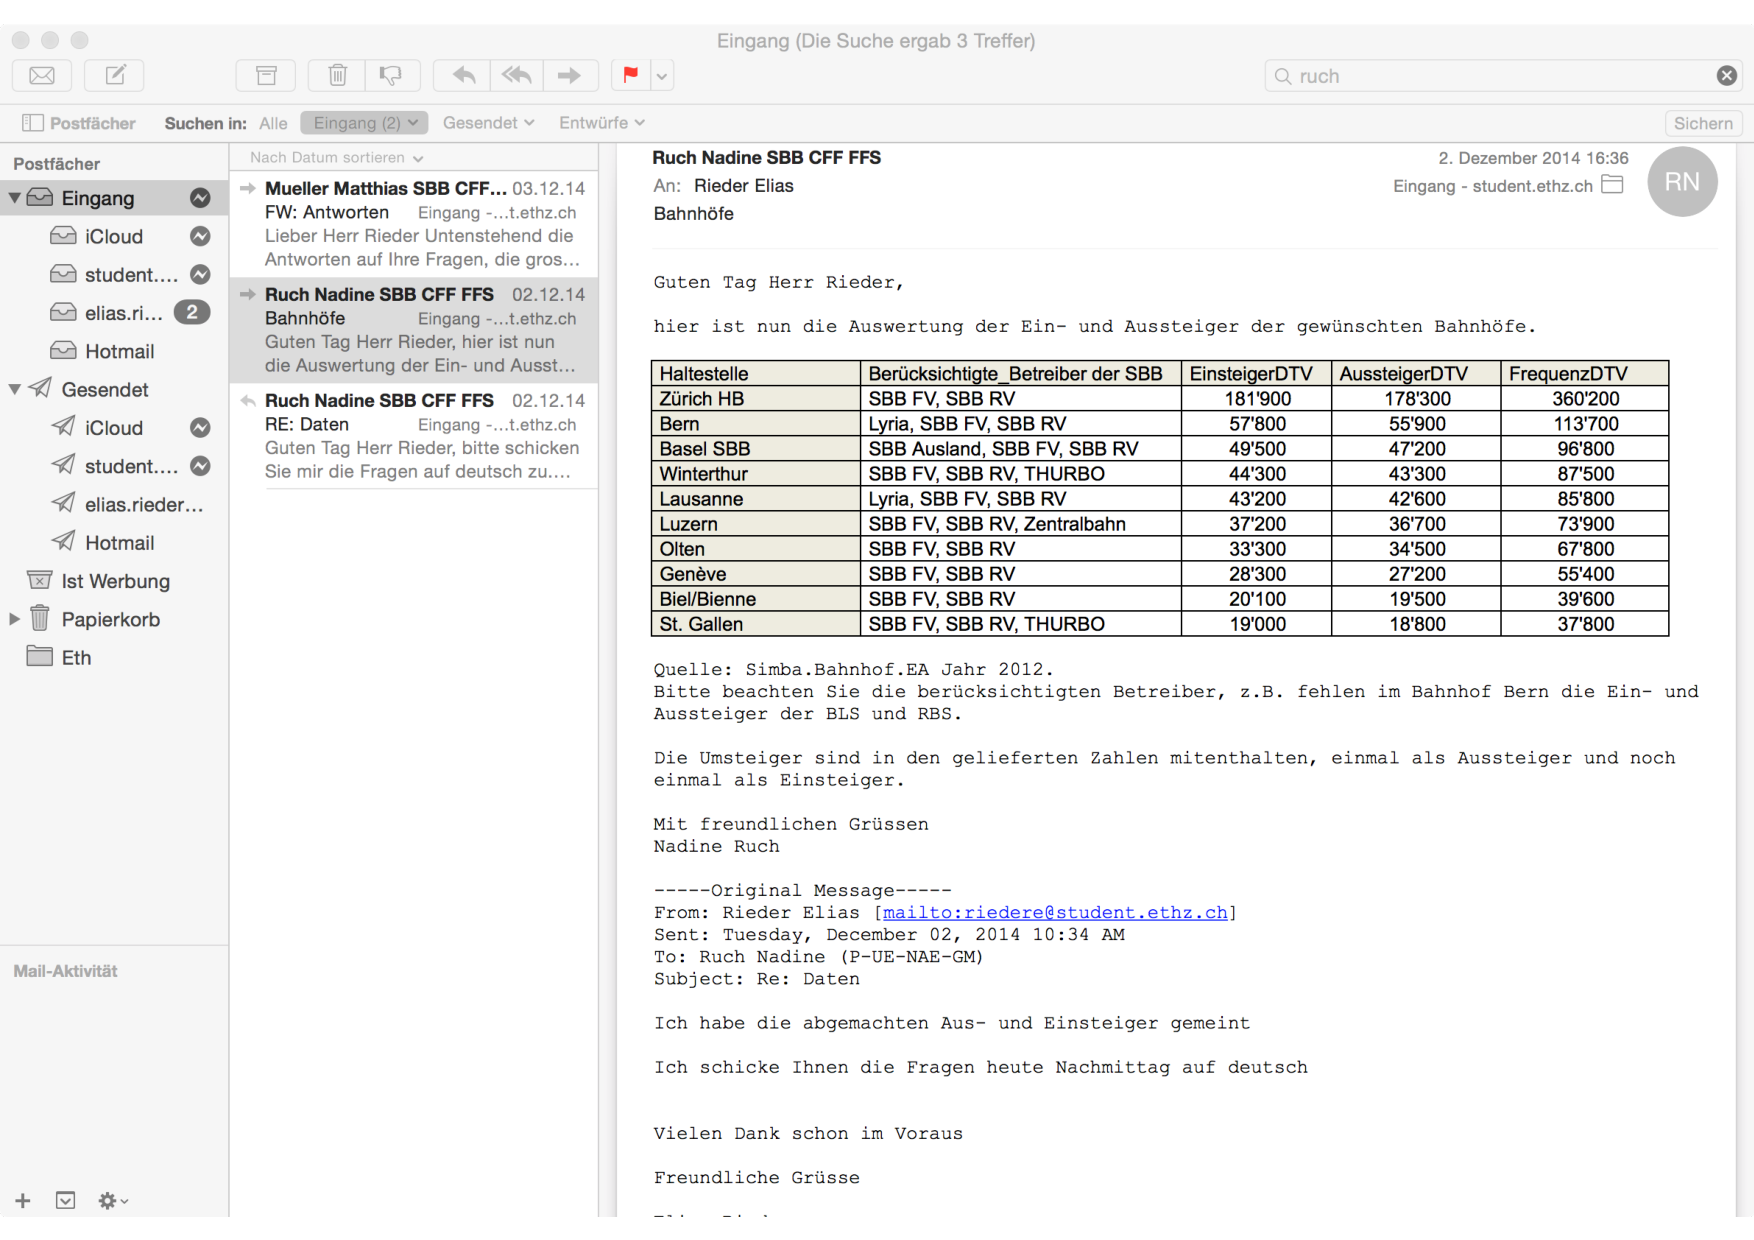
\includepdf[scale=0.8]{BoardingFF}
\end{figure}


\end{document}  
